
\documentclass{article}

%-------------------------------------------------------------------------------------------------------------
%  package
%--------------------------------------------------------------------------------------------------------------
%版面規劃(a4大小,上下左右距0.9inch)
\usepackage[a4paper,margin=0.9in]{geometry}
%作者資訊
\usepackage{authblk}
%中文化package
\usepackage{CJKutf8}

%分兩欄
\usepackage{multicol}
%分欄之後上圖需要有的package
\usepackage{float}
%然後若是需要在其中一欄上面加圖片=>[H大寫]
%要跨欄橫幅的圖片=>{figure*星號要加}[htbp]


%和插入圖片相關的package
\usepackage{graphicx}
\usepackage[tight]{subfigure}
\subfiguretopcaptrue
\usepackage{amsmath,booktabs,threeparttable,url, bm}
%\usepackage[hyphenbreaks]{breakurl}


%連結註腳網頁
\usepackage[colorlinks,linkcolor=blue]{hyperref}


%\newcommand{\cntext}{\begin{CJK}{UTF8}{bsmi}\end{CJK}}

\title{Assignment 8 of Computational Astrophysics in NTHU}
\author{Wei-Hsiang Yu 游惟翔}
\affil{Department of Physics, National Tsing Hua University, Hsinchu, Taiwan}

%-------------------------------------------------------------------------------------------------------------
%  文件開始
%--------------------------------------------------------------------------------------------------------------
\begin{document}

\begin{CJK}{UTF8}{bsmi}
%中文化需要加上此行才有title/author/date
\maketitle
\end{CJK}


%-------------------------------------------------------------------------------------------------------------
%  Programming Assignments
%--------------------------------------------------------------------------------------------------------------
\section{Programming Assignments}

%Q1---------------------------------------------------------------------
\subsection*{Q1 : Hydrodynamic PDE of heat equation.}


Heat equation
\begin{equation}
    u_{t}=u_{xx},\ 0\leq x\leq 1,\ t\geq 0
    \label{eq:heat}
\end{equation}

with initial condition
\begin{equation}
    u(0,x)= 2x,\ \mbox{ if }\ 0\leq x \leq 0.5
    \label{eq:ic}
\end{equation}
$$
    u(0,x)= 2-2x,\ \mbox{ if }\ 0.5\leq x \leq 1
$$

and boundary condition
\begin{equation}
    u(t,0)= 0, u(t,1)= 0, t\geq 0
    \label{eq:bc}
\end{equation}
\\

Using the fully discrete method to solve the heat equation.
\begin{equation}
    u_{t}\Rightarrow \frac{u_i^{n+1}-u_i^{n}}{\triangle t}
    \label{eq:tpart}
\end{equation}

\begin{equation}
    u_{xx}\Rightarrow \frac{u_{I+1}^{n}-2u_i^{n}+u_{i-1}^{n}}{(\triangle x)^2}
    \label{eq:xpart}
\end{equation}

and substitute Eq.\ref{eq:tpart} and Eq.\ref{eq:xpart} into heat equation Eq.\ref{eq:heat}, and transposition of term get Eq.\ref{eq:u}
$$
    \frac{u_i^{n+1}-u_i^{n}}{\triangle t}
    =
    \frac{u_{I+1}^{n}-2u_i^{n}+u_{i-1}^{n}}{(\triangle x)^2}
$$

\begin{equation}
    u_i^{n+1}=
    u_i^{n}+
    \frac{\triangle t}{(\triangle x)^2}
    (u_{i+1}^{n}-2u_i^{n}+u_{i-1}^{n})
    \label{eq:u}
\end{equation}

\subsubsection*{Q1.a\&b. : $\triangle t=0.0012$ / $\triangle t=0.0013$}
Given $\triangle x=0.05$ and calculate the solution from t=0 to t=0.06.

So \textbf{the number of points in x-direction will be 21}.
(need to record including the initial position x=0 to the final position x=1)

And we also need to consider the ghost zones for boundary condition \textbf{"ibuf=1"} because in Eq.\ref{eq:u}, there is u(i-1) and u(i+1) terms, which will face boundary problem when the update subroutine is run to the initial position x=0 (u(i-1)) and to the final position x=1 (u(i+1)).

The figure is showed in Fig.\ref{fig:pro1}, we can see that when $\triangle t=0.0012$, the solution will be smooth compared to the result when $\triangle t=0.0013$.

I consider it maybe relates to the CFL converge condition Eq.\ref{eq:cfl}.

\begin{equation}
    \triangle t \leq CFL (\triangle x)^2
    \label{eq:cfl}
\end{equation}

The Eq.\ref{eq:cfl} say that $\frac{\triangle t}{(\triangle x)^2}$ will be 0.48 when $\triangle t=0.0012$; 0.52 when $\triangle t=0.0013$.

So when we choose a larger time step with given space step, CFL value will also become larger, and based on CFL conclusion we can say that the numerical calculation will become unstable.



% %-------------------------------
\begin{figure}[h]
    \centering
    \subfigure[$\triangle t=0.0012$]{
        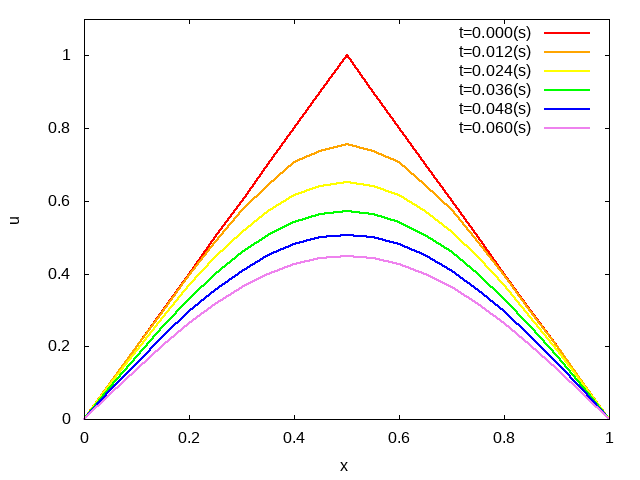
\includegraphics[scale=0.45]{t12_3.png}
        \label{fig:pro1_12}
    }
    \subfigure[$\triangle t=0.0013$]{
        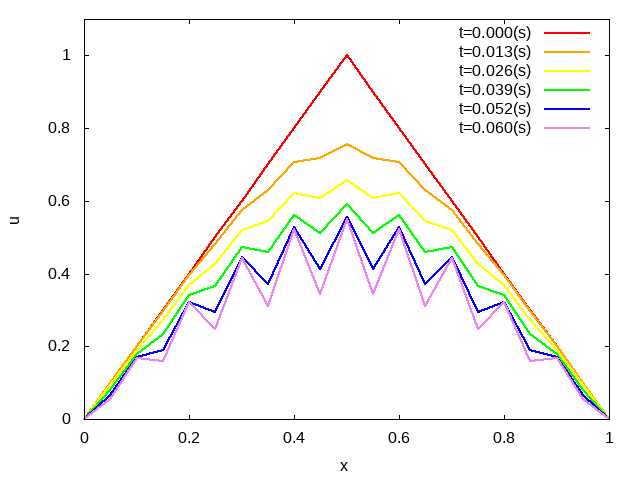
\includegraphics[scale=0.45]{t13_3.png}
        \label{fig:pro1_13} 
    }
    \caption{The solution from initial time to final time}
    \label{fig:pro1}
\end{figure}
% %-------------------------------







% \begin{thebibliography}{00}

% \bibitem{b1}
% Voyager 2 - Planetary Voyage\\
%  \href{https://web.archive.org/web/20131127192310/http://voyager.jpl.nasa.gov/science/planetary.html}{https://web.archive.org/web/20131127192310/http://voyager.jpl.nasa.gov/science/planetary.html}
 
% \bibitem{b2}
% Galileo - solar system exploration\\
%  \href{https://solarsystem.nasa.gov/missions/galileo/overview/}{https://solarsystem.nasa.gov/missions/galileo/overview/}

% \bibitem{b3}
% Gravity assist: The simple physics trick that’s allowed humanity to explore deep space\\
%  \href{https://blog.jatan.space/p/gravity-assist-the-simple-physics-trick-thats-allowed-humanity-to-explore-deep-space}{https://blog.jatan.space/p/gravity-assist-the-simple-physics-trick-thats-allowed-humanity-to-explore-deep-space}

% \end{thebibliography}

\end{document}

% \footnote{Lagrangian point:\href{https://en.wikipedia.org/wiki/Lagrange\_point}{https://en.wikipedia.org/wiki/Lagrange\_point}}


% %-------------------------------
% \begin{figure}[h]
%     \centering 
% 	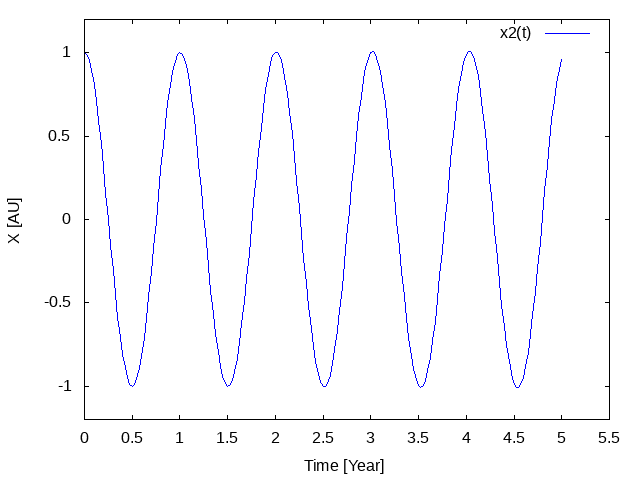
\includegraphics[scale=0.45]{pro1_x2.png}
% 	\caption{The trajectory of $m_1$ $m_2$ (when $m_2$ has a 1.25 factor of velocity).} %圖片註解
% 	\label{fig.pro1} %label 用這個就可以引用文章當中
% \end{figure}
% %-------------------------------

% %-------------------------------
% \begin{figure}[h]
%     \centering
%     \subfigure[dt=0.01yr]{
%         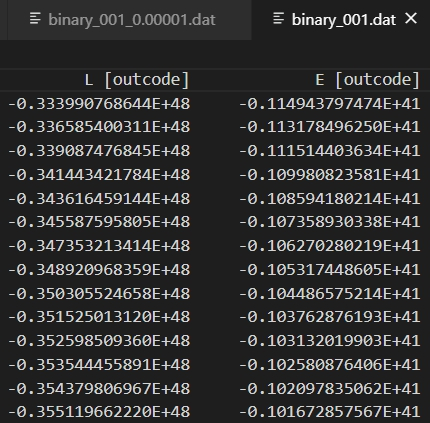
\includegraphics[scale=0.33]{01.jpg}
%         \label{01}
%     }
%     \subfigure[dt=0.001yr]{
%         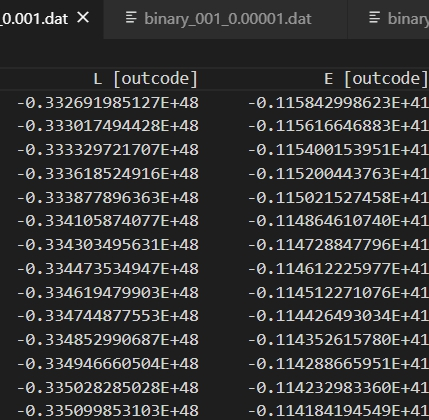
\includegraphics[scale=0.33]{001.jpg}
%         \label{001} 
%     }
%     \subfigure[dt=0.00001yr]{
%         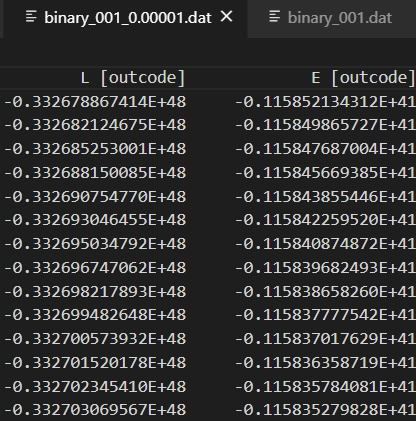
\includegraphics[scale=0.33]{00001.jpg}
%         \label{00001} 
%     }
%     \caption{L \& E in 0.01,0.001,0.00001 time step}
%     \label{fig:2c_dat}
% \end{figure}
% %-------------------------------